% Created by tikzDevice version 0.12.3.1 on 2022-08-18 15:37:37
% !TEX encoding = UTF-8 Unicode
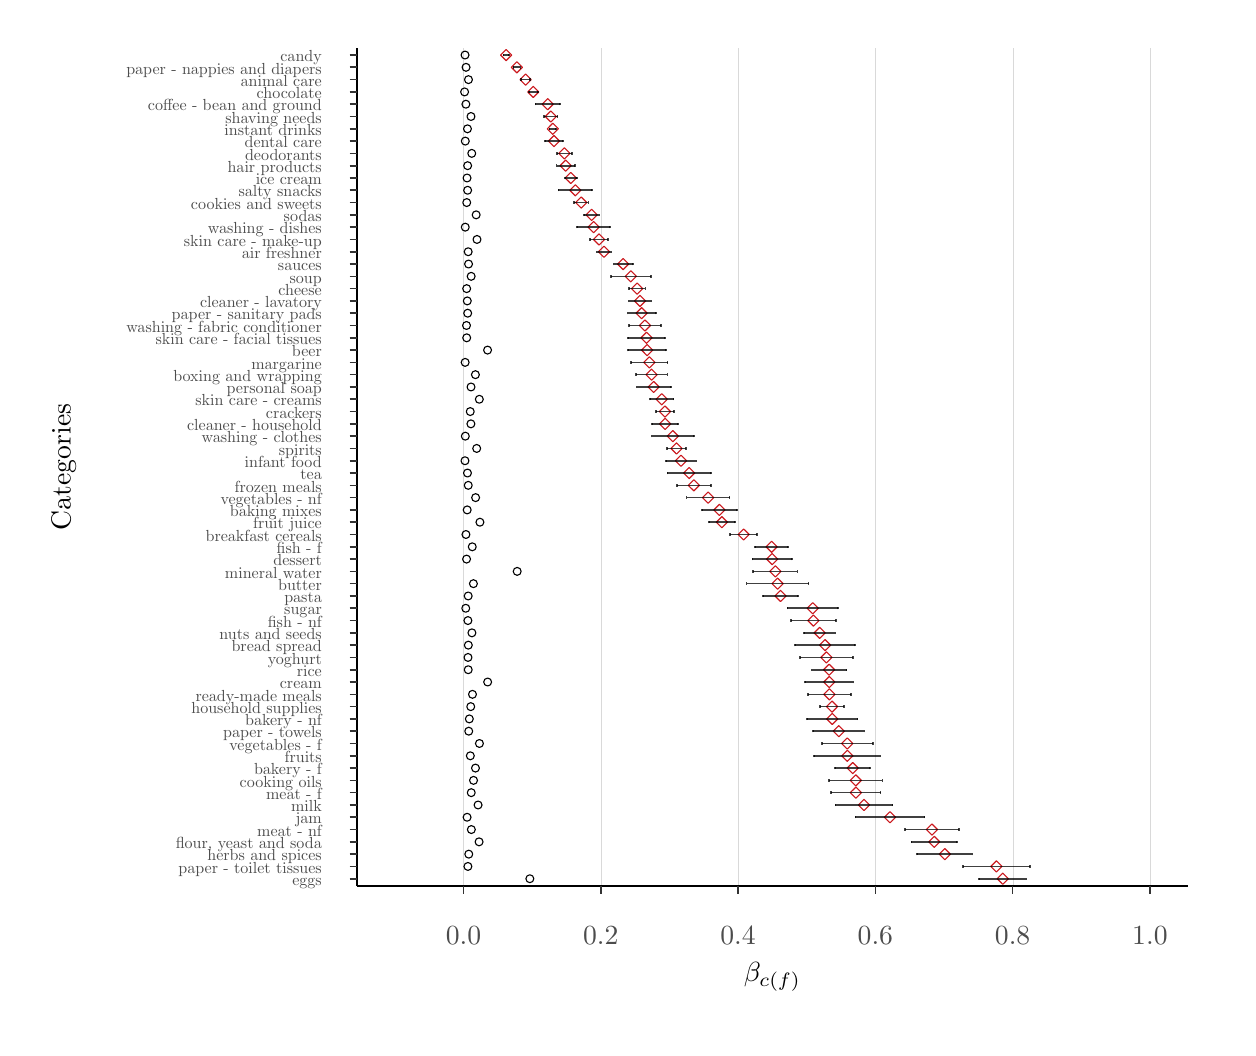
\begin{tikzpicture}[x=1pt,y=1pt]
\definecolor{fillColor}{RGB}{255,255,255}
\path[use as bounding box,fill=fillColor,fill opacity=0.00] (0,0) rectangle (433.62,361.35);
\begin{scope}
\path[clip] (  0.00,  0.00) rectangle (433.62,361.35);
\definecolor{drawColor}{RGB}{255,255,255}
\definecolor{fillColor}{RGB}{255,255,255}

\path[draw=drawColor,line width= 0.6pt,line join=round,line cap=round,fill=fillColor] (  0.00,  0.00) rectangle (433.62,361.35);
\end{scope}
\begin{scope}
\path[clip] (119.04, 51.15) rectangle (419.17,354.12);
\definecolor{drawColor}{RGB}{255,255,255}

\path[draw=drawColor,line width= 0.3pt,line join=round] (132.68, 51.15) --
	(132.68,354.12);

\path[draw=drawColor,line width= 0.3pt,line join=round] (182.29, 51.15) --
	(182.29,354.12);

\path[draw=drawColor,line width= 0.3pt,line join=round] (231.90, 51.15) --
	(231.90,354.12);

\path[draw=drawColor,line width= 0.3pt,line join=round] (281.51, 51.15) --
	(281.51,354.12);

\path[draw=drawColor,line width= 0.3pt,line join=round] (331.11, 51.15) --
	(331.11,354.12);

\path[draw=drawColor,line width= 0.3pt,line join=round] (380.72, 51.15) --
	(380.72,354.12);
\definecolor{drawColor}{gray}{0.85}

\path[draw=drawColor,line width= 0.1pt,line join=round] (157.49, 51.15) --
	(157.49,354.12);

\path[draw=drawColor,line width= 0.1pt,line join=round] (207.09, 51.15) --
	(207.09,354.12);

\path[draw=drawColor,line width= 0.1pt,line join=round] (256.70, 51.15) --
	(256.70,354.12);

\path[draw=drawColor,line width= 0.1pt,line join=round] (306.31, 51.15) --
	(306.31,354.12);

\path[draw=drawColor,line width= 0.1pt,line join=round] (355.92, 51.15) --
	(355.92,354.12);

\path[draw=drawColor,line width= 0.1pt,line join=round] (405.52, 51.15) --
	(405.52,354.12);
\definecolor{drawColor}{RGB}{0,0,0}

\path[draw=drawColor,line width= 0.4pt,line join=round,line cap=round] (159.18,280.38) circle (  1.43);

\path[draw=drawColor,line width= 0.4pt,line join=round,line cap=round] (159.28,342.57) circle (  1.43);

\path[draw=drawColor,line width= 0.4pt,line join=round,line cap=round] (161.81, 93.80) circle (  1.43);

\path[draw=drawColor,line width= 0.4pt,line join=round,line cap=round] (159.59,111.57) circle (  1.43);

\path[draw=drawColor,line width= 0.4pt,line join=round,line cap=round] (158.82,187.09) circle (  1.43);

\path[draw=drawColor,line width= 0.4pt,line join=round,line cap=round] (166.18,244.84) circle (  1.43);

\path[draw=drawColor,line width= 0.4pt,line join=round,line cap=round] (161.79,235.96) circle (  1.43);

\path[draw=drawColor,line width= 0.4pt,line join=round,line cap=round] (159.23,138.22) circle (  1.43);

\path[draw=drawColor,line width= 0.4pt,line join=round,line cap=round] (158.37,178.21) circle (  1.43);

\path[draw=drawColor,line width= 0.4pt,line join=round,line cap=round] (161.07,160.44) circle (  1.43);

\path[draw=drawColor,line width= 0.4pt,line join=round,line cap=round] (158.04,351.46) circle (  1.43);

\path[draw=drawColor,line width= 0.4pt,line join=round,line cap=round] (158.63,267.05) circle (  1.43);

\path[draw=drawColor,line width= 0.4pt,line join=round,line cap=round] (157.88,338.13) circle (  1.43);

\path[draw=drawColor,line width= 0.4pt,line join=round,line cap=round] (160.16,218.19) circle (  1.43);

\path[draw=drawColor,line width= 0.4pt,line join=round,line cap=round] (158.85,262.61) circle (  1.43);

\path[draw=drawColor,line width= 0.4pt,line join=round,line cap=round] (158.35,333.69) circle (  1.43);

\path[draw=drawColor,line width= 0.4pt,line join=round,line cap=round] (158.65,298.15) circle (  1.43);

\path[draw=drawColor,line width= 0.4pt,line join=round,line cap=round] (161.11, 89.36) circle (  1.43);

\path[draw=drawColor,line width= 0.4pt,line join=round,line cap=round] (159.92,222.63) circle (  1.43);

\path[draw=drawColor,line width= 0.4pt,line join=round,line cap=round] (166.21,124.90) circle (  1.43);

\path[draw=drawColor,line width= 0.4pt,line join=round,line cap=round] (158.13,320.36) circle (  1.43);

\path[draw=drawColor,line width= 0.4pt,line join=round,line cap=round] (160.47,315.92) circle (  1.43);

\path[draw=drawColor,line width= 0.4pt,line join=round,line cap=round] (158.59,169.32) circle (  1.43);

\path[draw=drawColor,line width= 0.4pt,line join=round,line cap=round] (181.46, 53.82) circle (  1.43);

\path[draw=drawColor,line width= 0.4pt,line join=round,line cap=round] (160.65,173.76) circle (  1.43);

\path[draw=drawColor,line width= 0.4pt,line join=round,line cap=round] (159.08,147.11) circle (  1.43);

\path[draw=drawColor,line width= 0.4pt,line join=round,line cap=round] (163.11, 67.15) circle (  1.43);

\path[draw=drawColor,line width= 0.4pt,line join=round,line cap=round] (159.20,195.97) circle (  1.43);

\path[draw=drawColor,line width= 0.4pt,line join=round,line cap=round] (163.42,182.65) circle (  1.43);

\path[draw=drawColor,line width= 0.4pt,line join=round,line cap=round] (159.95, 98.24) circle (  1.43);

\path[draw=drawColor,line width= 0.4pt,line join=round,line cap=round] (158.98,311.48) circle (  1.43);

\path[draw=drawColor,line width= 0.4pt,line join=round,line cap=round] (159.39, 62.70) circle (  1.43);

\path[draw=drawColor,line width= 0.4pt,line join=round,line cap=round] (160.10,116.01) circle (  1.43);

\path[draw=drawColor,line width= 0.4pt,line join=round,line cap=round] (158.76,307.03) circle (  1.43);

\path[draw=drawColor,line width= 0.4pt,line join=round,line cap=round] (158.02,204.86) circle (  1.43);

\path[draw=drawColor,line width= 0.4pt,line join=round,line cap=round] (158.92,324.80) circle (  1.43);

\path[draw=drawColor,line width= 0.4pt,line join=round,line cap=round] (158.78, 76.03) circle (  1.43);

\path[draw=drawColor,line width= 0.4pt,line join=round,line cap=round] (158.08,240.40) circle (  1.43);

\path[draw=drawColor,line width= 0.4pt,line join=round,line cap=round] (160.28, 84.92) circle (  1.43);

\path[draw=drawColor,line width= 0.4pt,line join=round,line cap=round] (160.32, 71.59) circle (  1.43);

\path[draw=drawColor,line width= 0.4pt,line join=round,line cap=round] (162.75, 80.47) circle (  1.43);

\path[draw=drawColor,line width= 0.4pt,line join=round,line cap=round] (176.88,164.88) circle (  1.43);

\path[draw=drawColor,line width= 0.4pt,line join=round,line cap=round] (160.53,142.67) circle (  1.43);

\path[draw=drawColor,line width= 0.4pt,line join=round,line cap=round] (158.40,347.02) circle (  1.43);

\path[draw=drawColor,line width= 0.4pt,line join=round,line cap=round] (159.00,258.17) circle (  1.43);

\path[draw=drawColor,line width= 0.4pt,line join=round,line cap=round] (159.08, 58.26) circle (  1.43);

\path[draw=drawColor,line width= 0.4pt,line join=round,line cap=round] (159.38,107.13) circle (  1.43);

\path[draw=drawColor,line width= 0.4pt,line join=round,line cap=round] (159.18,155.99) circle (  1.43);

\path[draw=drawColor,line width= 0.4pt,line join=round,line cap=round] (160.20,231.51) circle (  1.43);

\path[draw=drawColor,line width= 0.4pt,line join=round,line cap=round] (160.73,120.45) circle (  1.43);

\path[draw=drawColor,line width= 0.4pt,line join=round,line cap=round] (159.19,129.34) circle (  1.43);

\path[draw=drawColor,line width= 0.4pt,line join=round,line cap=round] (158.98,302.59) circle (  1.43);

\path[draw=drawColor,line width= 0.4pt,line join=round,line cap=round] (159.31,275.94) circle (  1.43);

\path[draw=drawColor,line width= 0.4pt,line join=round,line cap=round] (160.19,329.25) circle (  1.43);

\path[draw=drawColor,line width= 0.4pt,line join=round,line cap=round] (163.20,227.07) circle (  1.43);

\path[draw=drawColor,line width= 0.4pt,line join=round,line cap=round] (158.64,249.28) circle (  1.43);

\path[draw=drawColor,line width= 0.4pt,line join=round,line cap=round] (162.36,284.82) circle (  1.43);

\path[draw=drawColor,line width= 0.4pt,line join=round,line cap=round] (162.06,293.71) circle (  1.43);

\path[draw=drawColor,line width= 0.4pt,line join=round,line cap=round] (160.25,271.49) circle (  1.43);

\path[draw=drawColor,line width= 0.4pt,line join=round,line cap=round] (162.25,209.30) circle (  1.43);

\path[draw=drawColor,line width= 0.4pt,line join=round,line cap=round] (158.30,151.55) circle (  1.43);

\path[draw=drawColor,line width= 0.4pt,line join=round,line cap=round] (158.92,200.42) circle (  1.43);

\path[draw=drawColor,line width= 0.4pt,line join=round,line cap=round] (163.24,102.69) circle (  1.43);

\path[draw=drawColor,line width= 0.4pt,line join=round,line cap=round] (161.86,191.53) circle (  1.43);

\path[draw=drawColor,line width= 0.4pt,line join=round,line cap=round] (158.14,213.74) circle (  1.43);

\path[draw=drawColor,line width= 0.4pt,line join=round,line cap=round] (158.12,289.26) circle (  1.43);

\path[draw=drawColor,line width= 0.4pt,line join=round,line cap=round] (158.57,253.73) circle (  1.43);

\path[draw=drawColor,line width= 0.4pt,line join=round,line cap=round] (159.11,133.78) circle (  1.43);
\definecolor{drawColor}{RGB}{203,24,29}

\path[draw=drawColor,line width= 0.4pt,line join=round,line cap=round] (206.23,280.38) --
	(208.25,282.40) --
	(210.27,280.38) --
	(208.25,278.36) --
	cycle;

\path[draw=drawColor,line width= 0.4pt,line join=round,line cap=round] (177.90,342.57) --
	(179.92,344.59) --
	(181.94,342.57) --
	(179.92,340.56) --
	cycle;

\path[draw=drawColor,line width= 0.4pt,line join=round,line cap=round] (296.12, 93.80) --
	(298.13, 95.82) --
	(300.15, 93.80) --
	(298.13, 91.78) --
	cycle;

\path[draw=drawColor,line width= 0.4pt,line join=round,line cap=round] (288.70,111.57) --
	(290.72,113.59) --
	(292.74,111.57) --
	(290.72,109.55) --
	cycle;

\path[draw=drawColor,line width= 0.4pt,line join=round,line cap=round] (247.93,187.09) --
	(249.95,189.11) --
	(251.97,187.09) --
	(249.95,185.07) --
	cycle;

\path[draw=drawColor,line width= 0.4pt,line join=round,line cap=round] (221.83,244.84) --
	(223.84,246.86) --
	(225.86,244.84) --
	(223.84,242.82) --
	cycle;

\path[draw=drawColor,line width= 0.4pt,line join=round,line cap=round] (223.42,235.96) --
	(225.44,237.97) --
	(227.45,235.96) --
	(225.44,233.94) --
	cycle;

\path[draw=drawColor,line width= 0.4pt,line join=round,line cap=round] (286.11,138.22) --
	(288.13,140.24) --
	(290.15,138.22) --
	(288.13,136.21) --
	cycle;

\path[draw=drawColor,line width= 0.4pt,line join=round,line cap=round] (256.70,178.21) --
	(258.71,180.22) --
	(260.73,178.21) --
	(258.71,176.19) --
	cycle;

\path[draw=drawColor,line width= 0.4pt,line join=round,line cap=round] (268.95,160.44) --
	(270.97,162.45) --
	(272.99,160.44) --
	(270.97,158.42) --
	cycle;

\path[draw=drawColor,line width= 0.4pt,line join=round,line cap=round] (170.86,351.46) --
	(172.88,353.48) --
	(174.90,351.46) --
	(172.88,349.44) --
	cycle;

\path[draw=drawColor,line width= 0.4pt,line join=round,line cap=round] (218.19,267.05) --
	(220.21,269.07) --
	(222.22,267.05) --
	(220.21,265.04) --
	cycle;

\path[draw=drawColor,line width= 0.4pt,line join=round,line cap=round] (180.67,338.13) --
	(182.69,340.15) --
	(184.70,338.13) --
	(182.69,336.11) --
	cycle;

\path[draw=drawColor,line width= 0.4pt,line join=round,line cap=round] (228.32,218.19) --
	(230.34,220.20) --
	(232.35,218.19) --
	(230.34,216.17) --
	cycle;

\path[draw=drawColor,line width= 0.4pt,line join=round,line cap=round] (219.25,262.61) --
	(221.27,264.63) --
	(223.29,262.61) --
	(221.27,260.59) --
	cycle;

\path[draw=drawColor,line width= 0.4pt,line join=round,line cap=round] (185.91,333.69) --
	(187.92,335.71) --
	(189.94,333.69) --
	(187.92,331.67) --
	cycle;

\path[draw=drawColor,line width= 0.4pt,line join=round,line cap=round] (198.00,298.15) --
	(200.01,300.17) --
	(202.03,298.15) --
	(200.01,296.13) --
	cycle;

\path[draw=drawColor,line width= 0.4pt,line join=round,line cap=round] (297.22, 89.36) --
	(299.24, 91.38) --
	(301.26, 89.36) --
	(299.24, 87.34) --
	cycle;

\path[draw=drawColor,line width= 0.4pt,line join=round,line cap=round] (228.26,222.63) --
	(230.28,224.65) --
	(232.30,222.63) --
	(230.28,220.61) --
	cycle;

\path[draw=drawColor,line width= 0.4pt,line join=round,line cap=round] (287.64,124.90) --
	(289.66,126.91) --
	(291.67,124.90) --
	(289.66,122.88) --
	cycle;

\path[draw=drawColor,line width= 0.4pt,line join=round,line cap=round] (188.16,320.36) --
	(190.18,322.38) --
	(192.20,320.36) --
	(190.18,318.34) --
	cycle;

\path[draw=drawColor,line width= 0.4pt,line join=round,line cap=round] (191.93,315.92) --
	(193.95,317.94) --
	(195.97,315.92) --
	(193.95,313.90) --
	cycle;

\path[draw=drawColor,line width= 0.4pt,line join=round,line cap=round] (267.01,169.32) --
	(269.03,171.34) --
	(271.05,169.32) --
	(269.03,167.30) --
	cycle;

\path[draw=drawColor,line width= 0.4pt,line join=round,line cap=round] (350.34, 53.82) --
	(352.35, 55.84) --
	(354.37, 53.82) --
	(352.35, 51.80) --
	cycle;

\path[draw=drawColor,line width= 0.4pt,line join=round,line cap=round] (266.81,173.76) --
	(268.83,175.78) --
	(270.84,173.76) --
	(268.83,171.75) --
	cycle;

\path[draw=drawColor,line width= 0.4pt,line join=round,line cap=round] (281.90,147.11) --
	(283.92,149.13) --
	(285.94,147.11) --
	(283.92,145.09) --
	cycle;

\path[draw=drawColor,line width= 0.4pt,line join=round,line cap=round] (325.58, 67.15) --
	(327.59, 69.16) --
	(329.61, 67.15) --
	(327.59, 65.13) --
	cycle;

\path[draw=drawColor,line width= 0.4pt,line join=round,line cap=round] (238.71,195.97) --
	(240.73,197.99) --
	(242.74,195.97) --
	(240.73,193.96) --
	cycle;

\path[draw=drawColor,line width= 0.4pt,line join=round,line cap=round] (248.83,182.65) --
	(250.84,184.67) --
	(252.86,182.65) --
	(250.84,180.63) --
	cycle;

\path[draw=drawColor,line width= 0.4pt,line join=round,line cap=round] (294.16, 98.24) --
	(296.18,100.26) --
	(298.20, 98.24) --
	(296.18, 96.23) --
	cycle;

\path[draw=drawColor,line width= 0.4pt,line join=round,line cap=round] (192.38,311.48) --
	(194.40,313.49) --
	(196.42,311.48) --
	(194.40,309.46) --
	cycle;

\path[draw=drawColor,line width= 0.4pt,line join=round,line cap=round] (329.39, 62.70) --
	(331.41, 64.72) --
	(333.43, 62.70) --
	(331.41, 60.69) --
	cycle;

\path[draw=drawColor,line width= 0.4pt,line join=round,line cap=round] (288.63,116.01) --
	(290.65,118.03) --
	(292.66,116.01) --
	(290.65,113.99) --
	cycle;

\path[draw=drawColor,line width= 0.4pt,line join=round,line cap=round] (194.23,307.03) --
	(196.25,309.05) --
	(198.27,307.03) --
	(196.25,305.02) --
	cycle;

\path[draw=drawColor,line width= 0.4pt,line join=round,line cap=round] (234.07,204.86) --
	(236.08,206.88) --
	(238.10,204.86) --
	(236.08,202.84) --
	cycle;

\path[draw=drawColor,line width= 0.4pt,line join=round,line cap=round] (187.74,324.80) --
	(189.75,326.82) --
	(191.77,324.80) --
	(189.75,322.79) --
	cycle;

\path[draw=drawColor,line width= 0.4pt,line join=round,line cap=round] (309.59, 76.03) --
	(311.61, 78.05) --
	(313.62, 76.03) --
	(311.61, 74.01) --
	cycle;

\path[draw=drawColor,line width= 0.4pt,line join=round,line cap=round] (222.62,240.40) --
	(224.64,242.42) --
	(226.66,240.40) --
	(224.64,238.38) --
	cycle;

\path[draw=drawColor,line width= 0.4pt,line join=round,line cap=round] (297.25, 84.92) --
	(299.27, 86.93) --
	(301.28, 84.92) --
	(299.27, 82.90) --
	cycle;

\path[draw=drawColor,line width= 0.4pt,line join=round,line cap=round] (324.74, 71.59) --
	(326.76, 73.61) --
	(328.78, 71.59) --
	(326.76, 69.57) --
	cycle;

\path[draw=drawColor,line width= 0.4pt,line join=round,line cap=round] (300.19, 80.47) --
	(302.20, 82.49) --
	(304.22, 80.47) --
	(302.20, 78.46) --
	cycle;

\path[draw=drawColor,line width= 0.4pt,line join=round,line cap=round] (268.15,164.88) --
	(270.17,166.90) --
	(272.19,164.88) --
	(270.17,162.86) --
	cycle;

\path[draw=drawColor,line width= 0.4pt,line join=round,line cap=round] (284.18,142.67) --
	(286.20,144.68) --
	(288.22,142.67) --
	(286.20,140.65) --
	cycle;

\path[draw=drawColor,line width= 0.4pt,line join=round,line cap=round] (174.75,347.02) --
	(176.77,349.03) --
	(178.79,347.02) --
	(176.77,345.00) --
	cycle;

\path[draw=drawColor,line width= 0.4pt,line join=round,line cap=round] (219.83,258.17) --
	(221.85,260.19) --
	(223.87,258.17) --
	(221.85,256.15) --
	cycle;

\path[draw=drawColor,line width= 0.4pt,line join=round,line cap=round] (348.02, 58.26) --
	(350.04, 60.28) --
	(352.06, 58.26) --
	(350.04, 56.24) --
	cycle;

\path[draw=drawColor,line width= 0.4pt,line join=round,line cap=round] (291.09,107.13) --
	(293.11,109.14) --
	(295.12,107.13) --
	(293.11,105.11) --
	cycle;

\path[draw=drawColor,line width= 0.4pt,line join=round,line cap=round] (270.03,155.99) --
	(272.05,158.01) --
	(274.06,155.99) --
	(272.05,153.98) --
	cycle;

\path[draw=drawColor,line width= 0.4pt,line join=round,line cap=round] (224.17,231.51) --
	(226.19,233.53) --
	(228.21,231.51) --
	(226.19,229.50) --
	cycle;

\path[draw=drawColor,line width= 0.4pt,line join=round,line cap=round] (287.69,120.45) --
	(289.71,122.47) --
	(291.73,120.45) --
	(289.71,118.44) --
	cycle;

\path[draw=drawColor,line width= 0.4pt,line join=round,line cap=round] (287.58,129.34) --
	(289.60,131.36) --
	(291.62,129.34) --
	(289.60,127.32) --
	cycle;

\path[draw=drawColor,line width= 0.4pt,line join=round,line cap=round] (195.88,302.59) --
	(197.90,304.61) --
	(199.92,302.59) --
	(197.90,300.57) --
	cycle;

\path[draw=drawColor,line width= 0.4pt,line join=round,line cap=round] (213.15,275.94) --
	(215.17,277.95) --
	(217.18,275.94) --
	(215.17,273.92) --
	cycle;

\path[draw=drawColor,line width= 0.4pt,line join=round,line cap=round] (187.02,329.25) --
	(189.04,331.26) --
	(191.06,329.25) --
	(189.04,327.23) --
	cycle;

\path[draw=drawColor,line width= 0.4pt,line join=round,line cap=round] (227.09,227.07) --
	(229.11,229.09) --
	(231.13,227.07) --
	(229.11,225.05) --
	cycle;

\path[draw=drawColor,line width= 0.4pt,line join=round,line cap=round] (221.61,249.28) --
	(223.63,251.30) --
	(225.65,249.28) --
	(223.63,247.27) --
	cycle;

\path[draw=drawColor,line width= 0.4pt,line join=round,line cap=round] (204.45,284.82) --
	(206.46,286.84) --
	(208.48,284.82) --
	(206.46,282.80) --
	cycle;

\path[draw=drawColor,line width= 0.4pt,line join=round,line cap=round] (201.77,293.71) --
	(203.79,295.72) --
	(205.80,293.71) --
	(203.79,291.69) --
	cycle;

\path[draw=drawColor,line width= 0.4pt,line join=round,line cap=round] (215.92,271.49) --
	(217.94,273.51) --
	(219.95,271.49) --
	(217.94,269.48) --
	cycle;

\path[draw=drawColor,line width= 0.4pt,line join=round,line cap=round] (232.44,209.30) --
	(234.45,211.32) --
	(236.47,209.30) --
	(234.45,207.28) --
	cycle;

\path[draw=drawColor,line width= 0.4pt,line join=round,line cap=round] (281.67,151.55) --
	(283.69,153.57) --
	(285.71,151.55) --
	(283.69,149.53) --
	cycle;

\path[draw=drawColor,line width= 0.4pt,line join=round,line cap=round] (237.01,200.42) --
	(239.02,202.43) --
	(241.04,200.42) --
	(239.02,198.40) --
	cycle;

\path[draw=drawColor,line width= 0.4pt,line join=round,line cap=round] (294.12,102.69) --
	(296.14,104.70) --
	(298.16,102.69) --
	(296.14,100.67) --
	cycle;

\path[draw=drawColor,line width= 0.4pt,line join=round,line cap=round] (243.86,191.53) --
	(245.88,193.55) --
	(247.89,191.53) --
	(245.88,189.51) --
	cycle;

\path[draw=drawColor,line width= 0.4pt,line join=round,line cap=round] (231.10,213.74) --
	(233.12,215.76) --
	(235.14,213.74) --
	(233.12,211.73) --
	cycle;

\path[draw=drawColor,line width= 0.4pt,line join=round,line cap=round] (202.49,289.26) --
	(204.51,291.28) --
	(206.53,289.26) --
	(204.51,287.25) --
	cycle;

\path[draw=drawColor,line width= 0.4pt,line join=round,line cap=round] (221.03,253.73) --
	(223.05,255.74) --
	(225.07,253.73) --
	(223.05,251.71) --
	cycle;

\path[draw=drawColor,line width= 0.4pt,line join=round,line cap=round] (286.60,133.78) --
	(288.62,135.80) --
	(290.64,133.78) --
	(288.62,131.76) --
	cycle;
\definecolor{drawColor}{RGB}{0,0,0}

\path[draw=drawColor,draw opacity=0.75,line width= 0.6pt,line join=round] (210.94,279.94) --
	(210.94,280.82);

\path[draw=drawColor,draw opacity=0.75,line width= 0.6pt,line join=round] (210.94,280.38) --
	(205.56,280.38);

\path[draw=drawColor,draw opacity=0.75,line width= 0.6pt,line join=round] (205.56,279.94) --
	(205.56,280.82);

\path[draw=drawColor,draw opacity=0.75,line width= 0.6pt,line join=round] (181.48,342.13) --
	(181.48,343.02);

\path[draw=drawColor,draw opacity=0.75,line width= 0.6pt,line join=round] (181.48,342.57) --
	(178.35,342.57);

\path[draw=drawColor,draw opacity=0.75,line width= 0.6pt,line join=round] (178.35,342.13) --
	(178.35,343.02);

\path[draw=drawColor,draw opacity=0.75,line width= 0.6pt,line join=round] (304.44, 93.36) --
	(304.44, 94.24);

\path[draw=drawColor,draw opacity=0.75,line width= 0.6pt,line join=round] (304.44, 93.80) --
	(291.83, 93.80);

\path[draw=drawColor,draw opacity=0.75,line width= 0.6pt,line join=round] (291.83, 93.36) --
	(291.83, 94.24);

\path[draw=drawColor,draw opacity=0.75,line width= 0.6pt,line join=round] (299.87,111.13) --
	(299.87,112.01);

\path[draw=drawColor,draw opacity=0.75,line width= 0.6pt,line join=round] (299.87,111.57) --
	(281.57,111.57);

\path[draw=drawColor,draw opacity=0.75,line width= 0.6pt,line join=round] (281.57,111.13) --
	(281.57,112.01);

\path[draw=drawColor,draw opacity=0.75,line width= 0.6pt,line join=round] (256.20,186.65) --
	(256.20,187.53);

\path[draw=drawColor,draw opacity=0.75,line width= 0.6pt,line join=round] (256.20,187.09) --
	(243.70,187.09);

\path[draw=drawColor,draw opacity=0.75,line width= 0.6pt,line join=round] (243.70,186.65) --
	(243.70,187.53);

\path[draw=drawColor,draw opacity=0.75,line width= 0.6pt,line join=round] (230.68,244.40) --
	(230.68,245.29);

\path[draw=drawColor,draw opacity=0.75,line width= 0.6pt,line join=round] (230.68,244.84) --
	(217.01,244.84);

\path[draw=drawColor,draw opacity=0.75,line width= 0.6pt,line join=round] (217.01,244.40) --
	(217.01,245.29);

\path[draw=drawColor,draw opacity=0.75,line width= 0.6pt,line join=round] (231.16,235.51) --
	(231.16,236.40);

\path[draw=drawColor,draw opacity=0.75,line width= 0.6pt,line join=round] (231.16,235.96) --
	(219.71,235.96);

\path[draw=drawColor,draw opacity=0.75,line width= 0.6pt,line join=round] (219.71,235.51) --
	(219.71,236.40);

\path[draw=drawColor,draw opacity=0.75,line width= 0.6pt,line join=round] (299.06,137.78) --
	(299.06,138.67);

\path[draw=drawColor,draw opacity=0.75,line width= 0.6pt,line join=round] (299.06,138.22) --
	(277.20,138.22);

\path[draw=drawColor,draw opacity=0.75,line width= 0.6pt,line join=round] (277.20,137.78) --
	(277.20,138.67);

\path[draw=drawColor,draw opacity=0.75,line width= 0.6pt,line join=round] (263.59,177.76) --
	(263.59,178.65);

\path[draw=drawColor,draw opacity=0.75,line width= 0.6pt,line join=round] (263.59,178.21) --
	(253.83,178.21);

\path[draw=drawColor,draw opacity=0.75,line width= 0.6pt,line join=round] (253.83,177.76) --
	(253.83,178.65);

\path[draw=drawColor,draw opacity=0.75,line width= 0.6pt,line join=round] (282.19,159.99) --
	(282.19,160.88);

\path[draw=drawColor,draw opacity=0.75,line width= 0.6pt,line join=round] (282.19,160.44) --
	(259.75,160.44);

\path[draw=drawColor,draw opacity=0.75,line width= 0.6pt,line join=round] (259.75,159.99) --
	(259.75,160.88);

\path[draw=drawColor,draw opacity=0.75,line width= 0.6pt,line join=round] (173.88,351.01) --
	(173.88,351.90);

\path[draw=drawColor,draw opacity=0.75,line width= 0.6pt,line join=round] (173.88,351.46) --
	(171.88,351.46);

\path[draw=drawColor,draw opacity=0.75,line width= 0.6pt,line join=round] (171.88,351.01) --
	(171.88,351.90);

\path[draw=drawColor,draw opacity=0.75,line width= 0.6pt,line join=round] (223.21,266.61) --
	(223.21,267.50);

\path[draw=drawColor,draw opacity=0.75,line width= 0.6pt,line join=round] (223.21,267.05) --
	(217.20,267.05);

\path[draw=drawColor,draw opacity=0.75,line width= 0.6pt,line join=round] (217.20,266.61) --
	(217.20,267.50);

\path[draw=drawColor,draw opacity=0.75,line width= 0.6pt,line join=round] (184.33,337.69) --
	(184.33,338.57);

\path[draw=drawColor,draw opacity=0.75,line width= 0.6pt,line join=round] (184.33,338.13) --
	(181.04,338.13);

\path[draw=drawColor,draw opacity=0.75,line width= 0.6pt,line join=round] (181.04,337.69) --
	(181.04,338.57);

\path[draw=drawColor,draw opacity=0.75,line width= 0.6pt,line join=round] (235.03,217.74) --
	(235.03,218.63);

\path[draw=drawColor,draw opacity=0.75,line width= 0.6pt,line join=round] (235.03,218.19) --
	(225.65,218.19);

\path[draw=drawColor,draw opacity=0.75,line width= 0.6pt,line join=round] (225.65,217.74) --
	(225.65,218.63);

\path[draw=drawColor,draw opacity=0.75,line width= 0.6pt,line join=round] (225.40,262.17) --
	(225.40,263.05);

\path[draw=drawColor,draw opacity=0.75,line width= 0.6pt,line join=round] (225.40,262.61) --
	(217.13,262.61);

\path[draw=drawColor,draw opacity=0.75,line width= 0.6pt,line join=round] (217.13,262.17) --
	(217.13,263.05);

\path[draw=drawColor,draw opacity=0.75,line width= 0.6pt,line join=round] (192.38,333.24) --
	(192.38,334.13);

\path[draw=drawColor,draw opacity=0.75,line width= 0.6pt,line join=round] (192.38,333.69) --
	(183.47,333.69);

\path[draw=drawColor,draw opacity=0.75,line width= 0.6pt,line join=round] (183.47,333.24) --
	(183.47,334.13);

\path[draw=drawColor,draw opacity=0.75,line width= 0.6pt,line join=round] (202.63,297.70) --
	(202.63,298.59);

\path[draw=drawColor,draw opacity=0.75,line width= 0.6pt,line join=round] (202.63,298.15) --
	(197.40,298.15);

\path[draw=drawColor,draw opacity=0.75,line width= 0.6pt,line join=round] (197.40,297.70) --
	(197.40,298.59);

\path[draw=drawColor,draw opacity=0.75,line width= 0.6pt,line join=round] (308.88, 88.91) --
	(308.88, 89.80);

\path[draw=drawColor,draw opacity=0.75,line width= 0.6pt,line join=round] (308.88, 89.36) --
	(289.60, 89.36);

\path[draw=drawColor,draw opacity=0.75,line width= 0.6pt,line join=round] (289.60, 88.91) --
	(289.60, 89.80);

\path[draw=drawColor,draw opacity=0.75,line width= 0.6pt,line join=round] (233.44,222.18) --
	(233.44,223.07);

\path[draw=drawColor,draw opacity=0.75,line width= 0.6pt,line join=round] (233.44,222.63) --
	(227.12,222.63);

\path[draw=drawColor,draw opacity=0.75,line width= 0.6pt,line join=round] (227.12,222.18) --
	(227.12,223.07);

\path[draw=drawColor,draw opacity=0.75,line width= 0.6pt,line join=round] (298.38,124.45) --
	(298.38,125.34);

\path[draw=drawColor,draw opacity=0.75,line width= 0.6pt,line join=round] (298.38,124.90) --
	(280.93,124.90);

\path[draw=drawColor,draw opacity=0.75,line width= 0.6pt,line join=round] (280.93,124.45) --
	(280.93,125.34);

\path[draw=drawColor,draw opacity=0.75,line width= 0.6pt,line join=round] (193.50,319.92) --
	(193.50,320.81);

\path[draw=drawColor,draw opacity=0.75,line width= 0.6pt,line join=round] (193.50,320.36) --
	(186.85,320.36);

\path[draw=drawColor,draw opacity=0.75,line width= 0.6pt,line join=round] (186.85,319.92) --
	(186.85,320.81);

\path[draw=drawColor,draw opacity=0.75,line width= 0.6pt,line join=round] (196.74,315.47) --
	(196.74,316.36);

\path[draw=drawColor,draw opacity=0.75,line width= 0.6pt,line join=round] (196.74,315.92) --
	(191.17,315.92);

\path[draw=drawColor,draw opacity=0.75,line width= 0.6pt,line join=round] (191.17,315.47) --
	(191.17,316.36);

\path[draw=drawColor,draw opacity=0.75,line width= 0.6pt,line join=round] (276.20,168.88) --
	(276.20,169.76);

\path[draw=drawColor,draw opacity=0.75,line width= 0.6pt,line join=round] (276.20,169.32) --
	(261.86,169.32);

\path[draw=drawColor,draw opacity=0.75,line width= 0.6pt,line join=round] (261.86,168.88) --
	(261.86,169.76);

\path[draw=drawColor,draw opacity=0.75,line width= 0.6pt,line join=round] (360.90, 53.37) --
	(360.90, 54.26);

\path[draw=drawColor,draw opacity=0.75,line width= 0.6pt,line join=round] (360.90, 53.82) --
	(343.80, 53.82);

\path[draw=drawColor,draw opacity=0.75,line width= 0.6pt,line join=round] (343.80, 53.37) --
	(343.80, 54.26);

\path[draw=drawColor,draw opacity=0.75,line width= 0.6pt,line join=round] (274.84,173.32) --
	(274.84,174.21);

\path[draw=drawColor,draw opacity=0.75,line width= 0.6pt,line join=round] (274.84,173.76) --
	(262.81,173.76);

\path[draw=drawColor,draw opacity=0.75,line width= 0.6pt,line join=round] (262.81,173.32) --
	(262.81,174.21);

\path[draw=drawColor,draw opacity=0.75,line width= 0.6pt,line join=round] (292.03,146.66) --
	(292.03,147.55);

\path[draw=drawColor,draw opacity=0.75,line width= 0.6pt,line join=round] (292.03,147.11) --
	(275.81,147.11);

\path[draw=drawColor,draw opacity=0.75,line width= 0.6pt,line join=round] (275.81,146.66) --
	(275.81,147.55);

\path[draw=drawColor,draw opacity=0.75,line width= 0.6pt,line join=round] (335.83, 66.70) --
	(335.83, 67.59);

\path[draw=drawColor,draw opacity=0.75,line width= 0.6pt,line join=round] (335.83, 67.15) --
	(319.36, 67.15);

\path[draw=drawColor,draw opacity=0.75,line width= 0.6pt,line join=round] (319.36, 66.70) --
	(319.36, 67.59);

\path[draw=drawColor,draw opacity=0.75,line width= 0.6pt,line join=round] (246.86,195.53) --
	(246.86,196.42);

\path[draw=drawColor,draw opacity=0.75,line width= 0.6pt,line join=round] (246.86,195.97) --
	(234.59,195.97);

\path[draw=drawColor,draw opacity=0.75,line width= 0.6pt,line join=round] (234.59,195.53) --
	(234.59,196.42);

\path[draw=drawColor,draw opacity=0.75,line width= 0.6pt,line join=round] (255.61,182.20) --
	(255.61,183.09);

\path[draw=drawColor,draw opacity=0.75,line width= 0.6pt,line join=round] (255.61,182.65) --
	(246.08,182.65);

\path[draw=drawColor,draw opacity=0.75,line width= 0.6pt,line join=round] (246.08,182.20) --
	(246.08,183.09);

\path[draw=drawColor,draw opacity=0.75,line width= 0.6pt,line join=round] (308.12, 97.80) --
	(308.12, 98.69);

\path[draw=drawColor,draw opacity=0.75,line width= 0.6pt,line join=round] (308.12, 98.24) --
	(284.24, 98.24);

\path[draw=drawColor,draw opacity=0.75,line width= 0.6pt,line join=round] (284.24, 97.80) --
	(284.24, 98.69);

\path[draw=drawColor,draw opacity=0.75,line width= 0.6pt,line join=round] (197.66,311.03) --
	(197.66,311.92);

\path[draw=drawColor,draw opacity=0.75,line width= 0.6pt,line join=round] (197.66,311.48) --
	(191.14,311.48);

\path[draw=drawColor,draw opacity=0.75,line width= 0.6pt,line join=round] (191.14,311.03) --
	(191.14,311.92);

\path[draw=drawColor,draw opacity=0.75,line width= 0.6pt,line join=round] (341.40, 62.26) --
	(341.40, 63.15);

\path[draw=drawColor,draw opacity=0.75,line width= 0.6pt,line join=round] (341.40, 62.70) --
	(321.43, 62.70);

\path[draw=drawColor,draw opacity=0.75,line width= 0.6pt,line join=round] (321.43, 62.26) --
	(321.43, 63.15);

\path[draw=drawColor,draw opacity=0.75,line width= 0.6pt,line join=round] (294.95,115.57) --
	(294.95,116.46);

\path[draw=drawColor,draw opacity=0.75,line width= 0.6pt,line join=round] (294.95,116.01) --
	(286.34,116.01);

\path[draw=drawColor,draw opacity=0.75,line width= 0.6pt,line join=round] (286.34,115.57) --
	(286.34,116.46);

\path[draw=drawColor,draw opacity=0.75,line width= 0.6pt,line join=round] (198.38,306.59) --
	(198.38,307.48);

\path[draw=drawColor,draw opacity=0.75,line width= 0.6pt,line join=round] (198.38,307.03) --
	(194.12,307.03);

\path[draw=drawColor,draw opacity=0.75,line width= 0.6pt,line join=round] (194.12,306.59) --
	(194.12,307.48);

\path[draw=drawColor,draw opacity=0.75,line width= 0.6pt,line join=round] (241.62,204.42) --
	(241.62,205.30);

\path[draw=drawColor,draw opacity=0.75,line width= 0.6pt,line join=round] (241.62,204.86) --
	(230.55,204.86);

\path[draw=drawColor,draw opacity=0.75,line width= 0.6pt,line join=round] (230.55,204.42) --
	(230.55,205.30);

\path[draw=drawColor,draw opacity=0.75,line width= 0.6pt,line join=round] (190.98,324.36) --
	(190.98,325.25);

\path[draw=drawColor,draw opacity=0.75,line width= 0.6pt,line join=round] (190.98,324.80) --
	(188.53,324.80);

\path[draw=drawColor,draw opacity=0.75,line width= 0.6pt,line join=round] (188.53,324.36) --
	(188.53,325.25);

\path[draw=drawColor,draw opacity=0.75,line width= 0.6pt,line join=round] (324.11, 75.59) --
	(324.11, 76.48);

\path[draw=drawColor,draw opacity=0.75,line width= 0.6pt,line join=round] (324.11, 76.03) --
	(299.10, 76.03);

\path[draw=drawColor,draw opacity=0.75,line width= 0.6pt,line join=round] (299.10, 75.59) --
	(299.10, 76.48);

\path[draw=drawColor,draw opacity=0.75,line width= 0.6pt,line join=round] (231.24,239.95) --
	(231.24,240.84);

\path[draw=drawColor,draw opacity=0.75,line width= 0.6pt,line join=round] (231.24,240.40) --
	(218.04,240.40);

\path[draw=drawColor,draw opacity=0.75,line width= 0.6pt,line join=round] (218.04,239.95) --
	(218.04,240.84);

\path[draw=drawColor,draw opacity=0.75,line width= 0.6pt,line join=round] (308.22, 84.47) --
	(308.22, 85.36);

\path[draw=drawColor,draw opacity=0.75,line width= 0.6pt,line join=round] (308.22, 84.92) --
	(290.32, 84.92);

\path[draw=drawColor,draw opacity=0.75,line width= 0.6pt,line join=round] (290.32, 84.47) --
	(290.32, 85.36);

\path[draw=drawColor,draw opacity=0.75,line width= 0.6pt,line join=round] (336.60, 71.14) --
	(336.60, 72.03);

\path[draw=drawColor,draw opacity=0.75,line width= 0.6pt,line join=round] (336.60, 71.59) --
	(316.92, 71.59);

\path[draw=drawColor,draw opacity=0.75,line width= 0.6pt,line join=round] (316.92, 71.14) --
	(316.92, 72.03);

\path[draw=drawColor,draw opacity=0.75,line width= 0.6pt,line join=round] (312.51, 80.03) --
	(312.51, 80.92);

\path[draw=drawColor,draw opacity=0.75,line width= 0.6pt,line join=round] (312.51, 80.47) --
	(291.90, 80.47);

\path[draw=drawColor,draw opacity=0.75,line width= 0.6pt,line join=round] (291.90, 80.03) --
	(291.90, 80.92);

\path[draw=drawColor,draw opacity=0.75,line width= 0.6pt,line join=round] (278.15,164.43) --
	(278.15,165.32);

\path[draw=drawColor,draw opacity=0.75,line width= 0.6pt,line join=round] (278.15,164.88) --
	(262.19,164.88);

\path[draw=drawColor,draw opacity=0.75,line width= 0.6pt,line join=round] (262.19,164.43) --
	(262.19,165.32);

\path[draw=drawColor,draw opacity=0.75,line width= 0.6pt,line join=round] (291.90,142.22) --
	(291.90,143.11);

\path[draw=drawColor,draw opacity=0.75,line width= 0.6pt,line join=round] (291.90,142.67) --
	(280.49,142.67);

\path[draw=drawColor,draw opacity=0.75,line width= 0.6pt,line join=round] (280.49,142.22) --
	(280.49,143.11);

\path[draw=drawColor,draw opacity=0.75,line width= 0.6pt,line join=round] (178.06,346.57) --
	(178.06,347.46);

\path[draw=drawColor,draw opacity=0.75,line width= 0.6pt,line join=round] (178.06,347.02) --
	(175.49,347.02);

\path[draw=drawColor,draw opacity=0.75,line width= 0.6pt,line join=round] (175.49,346.57) --
	(175.49,347.46);

\path[draw=drawColor,draw opacity=0.75,line width= 0.6pt,line join=round] (226.94,257.72) --
	(226.94,258.61);

\path[draw=drawColor,draw opacity=0.75,line width= 0.6pt,line join=round] (226.94,258.17) --
	(216.76,258.17);

\path[draw=drawColor,draw opacity=0.75,line width= 0.6pt,line join=round] (216.76,257.72) --
	(216.76,258.61);

\path[draw=drawColor,draw opacity=0.75,line width= 0.6pt,line join=round] (362.21, 57.82) --
	(362.21, 58.71);

\path[draw=drawColor,draw opacity=0.75,line width= 0.6pt,line join=round] (362.21, 58.26) --
	(337.87, 58.26);

\path[draw=drawColor,draw opacity=0.75,line width= 0.6pt,line join=round] (337.87, 57.82) --
	(337.87, 58.71);

\path[draw=drawColor,draw opacity=0.75,line width= 0.6pt,line join=round] (302.33,106.68) --
	(302.33,107.57);

\path[draw=drawColor,draw opacity=0.75,line width= 0.6pt,line join=round] (302.33,107.13) --
	(283.88,107.13);

\path[draw=drawColor,draw opacity=0.75,line width= 0.6pt,line join=round] (283.88,106.68) --
	(283.88,107.57);

\path[draw=drawColor,draw opacity=0.75,line width= 0.6pt,line join=round] (278.34,155.55) --
	(278.34,156.44);

\path[draw=drawColor,draw opacity=0.75,line width= 0.6pt,line join=round] (278.34,155.99) --
	(265.75,155.99);

\path[draw=drawColor,draw opacity=0.75,line width= 0.6pt,line join=round] (265.75,155.55) --
	(265.75,156.44);

\path[draw=drawColor,draw opacity=0.75,line width= 0.6pt,line join=round] (232.36,231.07) --
	(232.36,231.96);

\path[draw=drawColor,draw opacity=0.75,line width= 0.6pt,line join=round] (232.36,231.51) --
	(220.02,231.51);

\path[draw=drawColor,draw opacity=0.75,line width= 0.6pt,line join=round] (220.02,231.07) --
	(220.02,231.96);

\path[draw=drawColor,draw opacity=0.75,line width= 0.6pt,line join=round] (297.50,120.01) --
	(297.50,120.90);

\path[draw=drawColor,draw opacity=0.75,line width= 0.6pt,line join=round] (297.50,120.45) --
	(281.92,120.45);

\path[draw=drawColor,draw opacity=0.75,line width= 0.6pt,line join=round] (281.92,120.01) --
	(281.92,120.90);

\path[draw=drawColor,draw opacity=0.75,line width= 0.6pt,line join=round] (295.91,128.90) --
	(295.91,129.78);

\path[draw=drawColor,draw opacity=0.75,line width= 0.6pt,line join=round] (295.91,129.34) --
	(283.29,129.34);

\path[draw=drawColor,draw opacity=0.75,line width= 0.6pt,line join=round] (283.29,128.90) --
	(283.29,129.78);

\path[draw=drawColor,draw opacity=0.75,line width= 0.6pt,line join=round] (204.01,302.15) --
	(204.01,303.04);

\path[draw=drawColor,draw opacity=0.75,line width= 0.6pt,line join=round] (204.01,302.59) --
	(191.79,302.59);

\path[draw=drawColor,draw opacity=0.75,line width= 0.6pt,line join=round] (191.79,302.15) --
	(191.79,303.04);

\path[draw=drawColor,draw opacity=0.75,line width= 0.6pt,line join=round] (218.64,275.49) --
	(218.64,276.38);

\path[draw=drawColor,draw opacity=0.75,line width= 0.6pt,line join=round] (218.64,275.94) --
	(211.70,275.94);

\path[draw=drawColor,draw opacity=0.75,line width= 0.6pt,line join=round] (211.70,275.49) --
	(211.70,276.38);

\path[draw=drawColor,draw opacity=0.75,line width= 0.6pt,line join=round] (191.48,328.80) --
	(191.48,329.69);

\path[draw=drawColor,draw opacity=0.75,line width= 0.6pt,line join=round] (191.48,329.25) --
	(186.60,329.25);

\path[draw=drawColor,draw opacity=0.75,line width= 0.6pt,line join=round] (186.60,328.80) --
	(186.60,329.69);

\path[draw=drawColor,draw opacity=0.75,line width= 0.6pt,line join=round] (233.38,226.63) --
	(233.38,227.52);

\path[draw=drawColor,draw opacity=0.75,line width= 0.6pt,line join=round] (233.38,227.07) --
	(224.83,227.07);

\path[draw=drawColor,draw opacity=0.75,line width= 0.6pt,line join=round] (224.83,226.63) --
	(224.83,227.52);

\path[draw=drawColor,draw opacity=0.75,line width= 0.6pt,line join=round] (230.22,248.84) --
	(230.22,249.73);

\path[draw=drawColor,draw opacity=0.75,line width= 0.6pt,line join=round] (230.22,249.28) --
	(217.03,249.28);

\path[draw=drawColor,draw opacity=0.75,line width= 0.6pt,line join=round] (217.03,248.84) --
	(217.03,249.73);

\path[draw=drawColor,draw opacity=0.75,line width= 0.6pt,line join=round] (209.74,284.38) --
	(209.74,285.27);

\path[draw=drawColor,draw opacity=0.75,line width= 0.6pt,line join=round] (209.74,284.82) --
	(203.18,284.82);

\path[draw=drawColor,draw opacity=0.75,line width= 0.6pt,line join=round] (203.18,284.38) --
	(203.18,285.27);

\path[draw=drawColor,draw opacity=0.75,line width= 0.6pt,line join=round] (206.60,293.26) --
	(206.60,294.15);

\path[draw=drawColor,draw opacity=0.75,line width= 0.6pt,line join=round] (206.60,293.71) --
	(200.97,293.71);

\path[draw=drawColor,draw opacity=0.75,line width= 0.6pt,line join=round] (200.97,293.26) --
	(200.97,294.15);

\path[draw=drawColor,draw opacity=0.75,line width= 0.6pt,line join=round] (225.20,271.05) --
	(225.20,271.94);

\path[draw=drawColor,draw opacity=0.75,line width= 0.6pt,line join=round] (225.20,271.49) --
	(210.68,271.49);

\path[draw=drawColor,draw opacity=0.75,line width= 0.6pt,line join=round] (210.68,271.05) --
	(210.68,271.94);

\path[draw=drawColor,draw opacity=0.75,line width= 0.6pt,line join=round] (237.91,208.86) --
	(237.91,209.75);

\path[draw=drawColor,draw opacity=0.75,line width= 0.6pt,line join=round] (237.91,209.30) --
	(231.00,209.30);

\path[draw=drawColor,draw opacity=0.75,line width= 0.6pt,line join=round] (231.00,208.86) --
	(231.00,209.75);

\path[draw=drawColor,draw opacity=0.75,line width= 0.6pt,line join=round] (292.89,151.11) --
	(292.89,152.00);

\path[draw=drawColor,draw opacity=0.75,line width= 0.6pt,line join=round] (292.89,151.55) --
	(274.50,151.55);

\path[draw=drawColor,draw opacity=0.75,line width= 0.6pt,line join=round] (274.50,151.11) --
	(274.50,152.00);

\path[draw=drawColor,draw opacity=0.75,line width= 0.6pt,line join=round] (246.88,199.97) --
	(246.88,200.86);

\path[draw=drawColor,draw opacity=0.75,line width= 0.6pt,line join=round] (246.88,200.42) --
	(231.17,200.42);

\path[draw=drawColor,draw opacity=0.75,line width= 0.6pt,line join=round] (231.17,199.97) --
	(231.17,200.86);

\path[draw=drawColor,draw opacity=0.75,line width= 0.6pt,line join=round] (305.36,102.24) --
	(305.36,103.13);

\path[draw=drawColor,draw opacity=0.75,line width= 0.6pt,line join=round] (305.36,102.69) --
	(286.91,102.69);

\path[draw=drawColor,draw opacity=0.75,line width= 0.6pt,line join=round] (286.91,102.24) --
	(286.91,103.13);

\path[draw=drawColor,draw opacity=0.75,line width= 0.6pt,line join=round] (253.65,191.09) --
	(253.65,191.98);

\path[draw=drawColor,draw opacity=0.75,line width= 0.6pt,line join=round] (253.65,191.53) --
	(238.11,191.53);

\path[draw=drawColor,draw opacity=0.75,line width= 0.6pt,line join=round] (238.11,191.09) --
	(238.11,191.98);

\path[draw=drawColor,draw opacity=0.75,line width= 0.6pt,line join=round] (240.80,213.30) --
	(240.80,214.19);

\path[draw=drawColor,draw opacity=0.75,line width= 0.6pt,line join=round] (240.80,213.74) --
	(225.44,213.74);

\path[draw=drawColor,draw opacity=0.75,line width= 0.6pt,line join=round] (225.44,213.30) --
	(225.44,214.19);

\path[draw=drawColor,draw opacity=0.75,line width= 0.6pt,line join=round] (210.42,288.82) --
	(210.42,289.71);

\path[draw=drawColor,draw opacity=0.75,line width= 0.6pt,line join=round] (210.42,289.26) --
	(198.60,289.26);

\path[draw=drawColor,draw opacity=0.75,line width= 0.6pt,line join=round] (198.60,288.82) --
	(198.60,289.71);

\path[draw=drawColor,draw opacity=0.75,line width= 0.6pt,line join=round] (228.88,253.28) --
	(228.88,254.17);

\path[draw=drawColor,draw opacity=0.75,line width= 0.6pt,line join=round] (228.88,253.73) --
	(217.22,253.73);

\path[draw=drawColor,draw opacity=0.75,line width= 0.6pt,line join=round] (217.22,253.28) --
	(217.22,254.17);

\path[draw=drawColor,draw opacity=0.75,line width= 0.6pt,line join=round] (298.27,133.34) --
	(298.27,134.23);

\path[draw=drawColor,draw opacity=0.75,line width= 0.6pt,line join=round] (298.27,133.78) --
	(278.97,133.78);

\path[draw=drawColor,draw opacity=0.75,line width= 0.6pt,line join=round] (278.97,133.34) --
	(278.97,134.23);
\end{scope}
\begin{scope}
\path[clip] (  0.00,  0.00) rectangle (433.62,361.35);
\definecolor{drawColor}{RGB}{0,0,0}

\path[draw=drawColor,line width= 0.6pt,line join=round] (119.04, 51.15) --
	(119.04,354.12);
\end{scope}
\begin{scope}
\path[clip] (  0.00,  0.00) rectangle (433.62,361.35);
\definecolor{drawColor}{gray}{0.30}

\node[text=drawColor,anchor=base east,inner sep=0pt, outer sep=0pt, scale=  0.58] at (106.29, 51.41) {eggs};

\node[text=drawColor,anchor=base east,inner sep=0pt, outer sep=0pt, scale=  0.58] at (106.29, 55.85) {paper - toilet tissues};

\node[text=drawColor,anchor=base east,inner sep=0pt, outer sep=0pt, scale=  0.58] at (106.29, 60.29) {herbs and spices};

\node[text=drawColor,anchor=base east,inner sep=0pt, outer sep=0pt, scale=  0.58] at (106.29, 64.74) {flour, yeast and soda};

\node[text=drawColor,anchor=base east,inner sep=0pt, outer sep=0pt, scale=  0.58] at (106.29, 69.18) {meat - nf};

\node[text=drawColor,anchor=base east,inner sep=0pt, outer sep=0pt, scale=  0.58] at (106.29, 73.62) {jam};

\node[text=drawColor,anchor=base east,inner sep=0pt, outer sep=0pt, scale=  0.58] at (106.29, 78.06) {milk};

\node[text=drawColor,anchor=base east,inner sep=0pt, outer sep=0pt, scale=  0.58] at (106.29, 82.50) {meat - f};

\node[text=drawColor,anchor=base east,inner sep=0pt, outer sep=0pt, scale=  0.58] at (106.29, 86.95) {cooking oils};

\node[text=drawColor,anchor=base east,inner sep=0pt, outer sep=0pt, scale=  0.58] at (106.29, 91.39) {bakery - f};

\node[text=drawColor,anchor=base east,inner sep=0pt, outer sep=0pt, scale=  0.58] at (106.29, 95.83) {fruits};

\node[text=drawColor,anchor=base east,inner sep=0pt, outer sep=0pt, scale=  0.58] at (106.29,100.27) {vegetables - f};

\node[text=drawColor,anchor=base east,inner sep=0pt, outer sep=0pt, scale=  0.58] at (106.29,104.72) {paper - towels};

\node[text=drawColor,anchor=base east,inner sep=0pt, outer sep=0pt, scale=  0.58] at (106.29,109.16) {bakery - nf};

\node[text=drawColor,anchor=base east,inner sep=0pt, outer sep=0pt, scale=  0.58] at (106.29,113.60) {household supplies};

\node[text=drawColor,anchor=base east,inner sep=0pt, outer sep=0pt, scale=  0.58] at (106.29,118.04) {ready-made meals};

\node[text=drawColor,anchor=base east,inner sep=0pt, outer sep=0pt, scale=  0.58] at (106.29,122.49) {cream};

\node[text=drawColor,anchor=base east,inner sep=0pt, outer sep=0pt, scale=  0.58] at (106.29,126.93) {rice};

\node[text=drawColor,anchor=base east,inner sep=0pt, outer sep=0pt, scale=  0.58] at (106.29,131.37) {yoghurt};

\node[text=drawColor,anchor=base east,inner sep=0pt, outer sep=0pt, scale=  0.58] at (106.29,135.81) {bread spread};

\node[text=drawColor,anchor=base east,inner sep=0pt, outer sep=0pt, scale=  0.58] at (106.29,140.26) {nuts and seeds};

\node[text=drawColor,anchor=base east,inner sep=0pt, outer sep=0pt, scale=  0.58] at (106.29,144.70) {fish - nf};

\node[text=drawColor,anchor=base east,inner sep=0pt, outer sep=0pt, scale=  0.58] at (106.29,149.14) {sugar};

\node[text=drawColor,anchor=base east,inner sep=0pt, outer sep=0pt, scale=  0.58] at (106.29,153.58) {pasta};

\node[text=drawColor,anchor=base east,inner sep=0pt, outer sep=0pt, scale=  0.58] at (106.29,158.02) {butter};

\node[text=drawColor,anchor=base east,inner sep=0pt, outer sep=0pt, scale=  0.58] at (106.29,162.47) {mineral water};

\node[text=drawColor,anchor=base east,inner sep=0pt, outer sep=0pt, scale=  0.58] at (106.29,166.91) {dessert};

\node[text=drawColor,anchor=base east,inner sep=0pt, outer sep=0pt, scale=  0.58] at (106.29,171.35) {fish - f};

\node[text=drawColor,anchor=base east,inner sep=0pt, outer sep=0pt, scale=  0.58] at (106.29,175.79) {breakfast cereals};

\node[text=drawColor,anchor=base east,inner sep=0pt, outer sep=0pt, scale=  0.58] at (106.29,180.24) {fruit juice};

\node[text=drawColor,anchor=base east,inner sep=0pt, outer sep=0pt, scale=  0.58] at (106.29,184.68) {baking mixes};

\node[text=drawColor,anchor=base east,inner sep=0pt, outer sep=0pt, scale=  0.58] at (106.29,189.12) {vegetables - nf};

\node[text=drawColor,anchor=base east,inner sep=0pt, outer sep=0pt, scale=  0.58] at (106.29,193.56) {frozen meals};

\node[text=drawColor,anchor=base east,inner sep=0pt, outer sep=0pt, scale=  0.58] at (106.29,198.01) {tea};

\node[text=drawColor,anchor=base east,inner sep=0pt, outer sep=0pt, scale=  0.58] at (106.29,202.45) {infant food};

\node[text=drawColor,anchor=base east,inner sep=0pt, outer sep=0pt, scale=  0.58] at (106.29,206.89) {spirits};

\node[text=drawColor,anchor=base east,inner sep=0pt, outer sep=0pt, scale=  0.58] at (106.29,211.33) {washing - clothes};

\node[text=drawColor,anchor=base east,inner sep=0pt, outer sep=0pt, scale=  0.58] at (106.29,215.78) {cleaner - household};

\node[text=drawColor,anchor=base east,inner sep=0pt, outer sep=0pt, scale=  0.58] at (106.29,220.22) {crackers};

\node[text=drawColor,anchor=base east,inner sep=0pt, outer sep=0pt, scale=  0.58] at (106.29,224.66) {skin care - creams};

\node[text=drawColor,anchor=base east,inner sep=0pt, outer sep=0pt, scale=  0.58] at (106.29,229.10) {personal soap};

\node[text=drawColor,anchor=base east,inner sep=0pt, outer sep=0pt, scale=  0.58] at (106.29,233.55) {boxing and wrapping};

\node[text=drawColor,anchor=base east,inner sep=0pt, outer sep=0pt, scale=  0.58] at (106.29,237.99) {margarine};

\node[text=drawColor,anchor=base east,inner sep=0pt, outer sep=0pt, scale=  0.58] at (106.29,242.43) {beer};

\node[text=drawColor,anchor=base east,inner sep=0pt, outer sep=0pt, scale=  0.58] at (106.29,246.87) {skin care - facial tissues};

\node[text=drawColor,anchor=base east,inner sep=0pt, outer sep=0pt, scale=  0.58] at (106.29,251.31) {washing - fabric conditioner};

\node[text=drawColor,anchor=base east,inner sep=0pt, outer sep=0pt, scale=  0.58] at (106.29,255.76) {paper - sanitary pads};

\node[text=drawColor,anchor=base east,inner sep=0pt, outer sep=0pt, scale=  0.58] at (106.29,260.20) {cleaner - lavatory};

\node[text=drawColor,anchor=base east,inner sep=0pt, outer sep=0pt, scale=  0.58] at (106.29,264.64) {cheese};

\node[text=drawColor,anchor=base east,inner sep=0pt, outer sep=0pt, scale=  0.58] at (106.29,269.08) {soup};

\node[text=drawColor,anchor=base east,inner sep=0pt, outer sep=0pt, scale=  0.58] at (106.29,273.53) {sauces};

\node[text=drawColor,anchor=base east,inner sep=0pt, outer sep=0pt, scale=  0.58] at (106.29,277.97) {air freshner};

\node[text=drawColor,anchor=base east,inner sep=0pt, outer sep=0pt, scale=  0.58] at (106.29,282.41) {skin care - make-up};

\node[text=drawColor,anchor=base east,inner sep=0pt, outer sep=0pt, scale=  0.58] at (106.29,286.85) {washing - dishes};

\node[text=drawColor,anchor=base east,inner sep=0pt, outer sep=0pt, scale=  0.58] at (106.29,291.30) {sodas};

\node[text=drawColor,anchor=base east,inner sep=0pt, outer sep=0pt, scale=  0.58] at (106.29,295.74) {cookies and sweets};

\node[text=drawColor,anchor=base east,inner sep=0pt, outer sep=0pt, scale=  0.58] at (106.29,300.18) {salty snacks};

\node[text=drawColor,anchor=base east,inner sep=0pt, outer sep=0pt, scale=  0.58] at (106.29,304.62) {ice cream};

\node[text=drawColor,anchor=base east,inner sep=0pt, outer sep=0pt, scale=  0.58] at (106.29,309.07) {hair products};

\node[text=drawColor,anchor=base east,inner sep=0pt, outer sep=0pt, scale=  0.58] at (106.29,313.51) {deodorants};

\node[text=drawColor,anchor=base east,inner sep=0pt, outer sep=0pt, scale=  0.58] at (106.29,317.95) {dental care};

\node[text=drawColor,anchor=base east,inner sep=0pt, outer sep=0pt, scale=  0.58] at (106.29,322.39) {instant drinks};

\node[text=drawColor,anchor=base east,inner sep=0pt, outer sep=0pt, scale=  0.58] at (106.29,326.83) {shaving needs};

\node[text=drawColor,anchor=base east,inner sep=0pt, outer sep=0pt, scale=  0.58] at (106.29,331.28) {coffee - bean and ground};

\node[text=drawColor,anchor=base east,inner sep=0pt, outer sep=0pt, scale=  0.58] at (106.29,335.72) {chocolate};

\node[text=drawColor,anchor=base east,inner sep=0pt, outer sep=0pt, scale=  0.58] at (106.29,340.16) {animal care};

\node[text=drawColor,anchor=base east,inner sep=0pt, outer sep=0pt, scale=  0.58] at (106.29,344.60) {paper - nappies and diapers};

\node[text=drawColor,anchor=base east,inner sep=0pt, outer sep=0pt, scale=  0.58] at (106.29,349.05) {candy};
\end{scope}
\begin{scope}
\path[clip] (  0.00,  0.00) rectangle (433.62,361.35);
\definecolor{drawColor}{gray}{0.20}

\path[draw=drawColor,line width= 0.6pt,line join=round] (116.29, 53.82) --
	(119.04, 53.82);

\path[draw=drawColor,line width= 0.6pt,line join=round] (116.29, 58.26) --
	(119.04, 58.26);

\path[draw=drawColor,line width= 0.6pt,line join=round] (116.29, 62.70) --
	(119.04, 62.70);

\path[draw=drawColor,line width= 0.6pt,line join=round] (116.29, 67.15) --
	(119.04, 67.15);

\path[draw=drawColor,line width= 0.6pt,line join=round] (116.29, 71.59) --
	(119.04, 71.59);

\path[draw=drawColor,line width= 0.6pt,line join=round] (116.29, 76.03) --
	(119.04, 76.03);

\path[draw=drawColor,line width= 0.6pt,line join=round] (116.29, 80.47) --
	(119.04, 80.47);

\path[draw=drawColor,line width= 0.6pt,line join=round] (116.29, 84.92) --
	(119.04, 84.92);

\path[draw=drawColor,line width= 0.6pt,line join=round] (116.29, 89.36) --
	(119.04, 89.36);

\path[draw=drawColor,line width= 0.6pt,line join=round] (116.29, 93.80) --
	(119.04, 93.80);

\path[draw=drawColor,line width= 0.6pt,line join=round] (116.29, 98.24) --
	(119.04, 98.24);

\path[draw=drawColor,line width= 0.6pt,line join=round] (116.29,102.69) --
	(119.04,102.69);

\path[draw=drawColor,line width= 0.6pt,line join=round] (116.29,107.13) --
	(119.04,107.13);

\path[draw=drawColor,line width= 0.6pt,line join=round] (116.29,111.57) --
	(119.04,111.57);

\path[draw=drawColor,line width= 0.6pt,line join=round] (116.29,116.01) --
	(119.04,116.01);

\path[draw=drawColor,line width= 0.6pt,line join=round] (116.29,120.45) --
	(119.04,120.45);

\path[draw=drawColor,line width= 0.6pt,line join=round] (116.29,124.90) --
	(119.04,124.90);

\path[draw=drawColor,line width= 0.6pt,line join=round] (116.29,129.34) --
	(119.04,129.34);

\path[draw=drawColor,line width= 0.6pt,line join=round] (116.29,133.78) --
	(119.04,133.78);

\path[draw=drawColor,line width= 0.6pt,line join=round] (116.29,138.22) --
	(119.04,138.22);

\path[draw=drawColor,line width= 0.6pt,line join=round] (116.29,142.67) --
	(119.04,142.67);

\path[draw=drawColor,line width= 0.6pt,line join=round] (116.29,147.11) --
	(119.04,147.11);

\path[draw=drawColor,line width= 0.6pt,line join=round] (116.29,151.55) --
	(119.04,151.55);

\path[draw=drawColor,line width= 0.6pt,line join=round] (116.29,155.99) --
	(119.04,155.99);

\path[draw=drawColor,line width= 0.6pt,line join=round] (116.29,160.44) --
	(119.04,160.44);

\path[draw=drawColor,line width= 0.6pt,line join=round] (116.29,164.88) --
	(119.04,164.88);

\path[draw=drawColor,line width= 0.6pt,line join=round] (116.29,169.32) --
	(119.04,169.32);

\path[draw=drawColor,line width= 0.6pt,line join=round] (116.29,173.76) --
	(119.04,173.76);

\path[draw=drawColor,line width= 0.6pt,line join=round] (116.29,178.21) --
	(119.04,178.21);

\path[draw=drawColor,line width= 0.6pt,line join=round] (116.29,182.65) --
	(119.04,182.65);

\path[draw=drawColor,line width= 0.6pt,line join=round] (116.29,187.09) --
	(119.04,187.09);

\path[draw=drawColor,line width= 0.6pt,line join=round] (116.29,191.53) --
	(119.04,191.53);

\path[draw=drawColor,line width= 0.6pt,line join=round] (116.29,195.97) --
	(119.04,195.97);

\path[draw=drawColor,line width= 0.6pt,line join=round] (116.29,200.42) --
	(119.04,200.42);

\path[draw=drawColor,line width= 0.6pt,line join=round] (116.29,204.86) --
	(119.04,204.86);

\path[draw=drawColor,line width= 0.6pt,line join=round] (116.29,209.30) --
	(119.04,209.30);

\path[draw=drawColor,line width= 0.6pt,line join=round] (116.29,213.74) --
	(119.04,213.74);

\path[draw=drawColor,line width= 0.6pt,line join=round] (116.29,218.19) --
	(119.04,218.19);

\path[draw=drawColor,line width= 0.6pt,line join=round] (116.29,222.63) --
	(119.04,222.63);

\path[draw=drawColor,line width= 0.6pt,line join=round] (116.29,227.07) --
	(119.04,227.07);

\path[draw=drawColor,line width= 0.6pt,line join=round] (116.29,231.51) --
	(119.04,231.51);

\path[draw=drawColor,line width= 0.6pt,line join=round] (116.29,235.96) --
	(119.04,235.96);

\path[draw=drawColor,line width= 0.6pt,line join=round] (116.29,240.40) --
	(119.04,240.40);

\path[draw=drawColor,line width= 0.6pt,line join=round] (116.29,244.84) --
	(119.04,244.84);

\path[draw=drawColor,line width= 0.6pt,line join=round] (116.29,249.28) --
	(119.04,249.28);

\path[draw=drawColor,line width= 0.6pt,line join=round] (116.29,253.73) --
	(119.04,253.73);

\path[draw=drawColor,line width= 0.6pt,line join=round] (116.29,258.17) --
	(119.04,258.17);

\path[draw=drawColor,line width= 0.6pt,line join=round] (116.29,262.61) --
	(119.04,262.61);

\path[draw=drawColor,line width= 0.6pt,line join=round] (116.29,267.05) --
	(119.04,267.05);

\path[draw=drawColor,line width= 0.6pt,line join=round] (116.29,271.49) --
	(119.04,271.49);

\path[draw=drawColor,line width= 0.6pt,line join=round] (116.29,275.94) --
	(119.04,275.94);

\path[draw=drawColor,line width= 0.6pt,line join=round] (116.29,280.38) --
	(119.04,280.38);

\path[draw=drawColor,line width= 0.6pt,line join=round] (116.29,284.82) --
	(119.04,284.82);

\path[draw=drawColor,line width= 0.6pt,line join=round] (116.29,289.26) --
	(119.04,289.26);

\path[draw=drawColor,line width= 0.6pt,line join=round] (116.29,293.71) --
	(119.04,293.71);

\path[draw=drawColor,line width= 0.6pt,line join=round] (116.29,298.15) --
	(119.04,298.15);

\path[draw=drawColor,line width= 0.6pt,line join=round] (116.29,302.59) --
	(119.04,302.59);

\path[draw=drawColor,line width= 0.6pt,line join=round] (116.29,307.03) --
	(119.04,307.03);

\path[draw=drawColor,line width= 0.6pt,line join=round] (116.29,311.48) --
	(119.04,311.48);

\path[draw=drawColor,line width= 0.6pt,line join=round] (116.29,315.92) --
	(119.04,315.92);

\path[draw=drawColor,line width= 0.6pt,line join=round] (116.29,320.36) --
	(119.04,320.36);

\path[draw=drawColor,line width= 0.6pt,line join=round] (116.29,324.80) --
	(119.04,324.80);

\path[draw=drawColor,line width= 0.6pt,line join=round] (116.29,329.25) --
	(119.04,329.25);

\path[draw=drawColor,line width= 0.6pt,line join=round] (116.29,333.69) --
	(119.04,333.69);

\path[draw=drawColor,line width= 0.6pt,line join=round] (116.29,338.13) --
	(119.04,338.13);

\path[draw=drawColor,line width= 0.6pt,line join=round] (116.29,342.57) --
	(119.04,342.57);

\path[draw=drawColor,line width= 0.6pt,line join=round] (116.29,347.02) --
	(119.04,347.02);

\path[draw=drawColor,line width= 0.6pt,line join=round] (116.29,351.46) --
	(119.04,351.46);
\end{scope}
\begin{scope}
\path[clip] (  0.00,  0.00) rectangle (433.62,361.35);
\definecolor{drawColor}{RGB}{0,0,0}

\path[draw=drawColor,line width= 0.6pt,line join=round] (119.04, 51.15) --
	(419.17, 51.15);
\end{scope}
\begin{scope}
\path[clip] (  0.00,  0.00) rectangle (433.62,361.35);
\definecolor{drawColor}{gray}{0.20}

\path[draw=drawColor,line width= 0.6pt,line join=round] (157.49, 48.40) --
	(157.49, 51.15);

\path[draw=drawColor,line width= 0.6pt,line join=round] (207.09, 48.40) --
	(207.09, 51.15);

\path[draw=drawColor,line width= 0.6pt,line join=round] (256.70, 48.40) --
	(256.70, 51.15);

\path[draw=drawColor,line width= 0.6pt,line join=round] (306.31, 48.40) --
	(306.31, 51.15);

\path[draw=drawColor,line width= 0.6pt,line join=round] (355.92, 48.40) --
	(355.92, 51.15);

\path[draw=drawColor,line width= 0.6pt,line join=round] (405.52, 48.40) --
	(405.52, 51.15);
\end{scope}
\begin{scope}
\path[clip] (  0.00,  0.00) rectangle (433.62,361.35);
\definecolor{drawColor}{gray}{0.30}

\node[text=drawColor,anchor=base,inner sep=0pt, outer sep=0pt, scale=  1.00] at (157.49, 30.14) {0.0};

\node[text=drawColor,anchor=base,inner sep=0pt, outer sep=0pt, scale=  1.00] at (207.09, 30.14) {0.2};

\node[text=drawColor,anchor=base,inner sep=0pt, outer sep=0pt, scale=  1.00] at (256.70, 30.14) {0.4};

\node[text=drawColor,anchor=base,inner sep=0pt, outer sep=0pt, scale=  1.00] at (306.31, 30.14) {0.6};

\node[text=drawColor,anchor=base,inner sep=0pt, outer sep=0pt, scale=  1.00] at (355.92, 30.14) {0.8};

\node[text=drawColor,anchor=base,inner sep=0pt, outer sep=0pt, scale=  1.00] at (405.52, 30.14) {1.0};
\end{scope}
\begin{scope}
\path[clip] (  0.00,  0.00) rectangle (433.62,361.35);
\definecolor{drawColor}{RGB}{0,0,0}

\node[text=drawColor,anchor=base,inner sep=0pt, outer sep=0pt, scale=  1.00] at (269.10, 16.79) {$\beta_{c(f)}$};
\end{scope}
\begin{scope}
\path[clip] (  0.00,  0.00) rectangle (433.62,361.35);
\definecolor{drawColor}{RGB}{0,0,0}

\node[text=drawColor,rotate= 90.00,anchor=base,inner sep=0pt, outer sep=0pt, scale=  1.00] at ( 15.49,202.64) {Categories};
\end{scope}
\end{tikzpicture}
